 \documentclass[a4paper,11pt]{article}

\usepackage{amsmath}
\usepackage{amssymb}
\usepackage{amsthm}
\usepackage{graphicx}
\usepackage{caption}
\usepackage{subcaption}

\newtheorem{thm}{Theorem}
\newtheorem{lem}{Lemma}

\newcommand{\beq}{\begin{equation}}
\newcommand{\eeq}{\end{equation}}

\newcommand{\ba}{\begin{array}}
\newcommand{\ea}{\end{array}}

\newcommand{\bea}{\begin{eqnarray}}
\newcommand{\eea}{\end{eqnarray}}

\newcommand{\bc}{\begin{center}}
\newcommand{\ec}{\end{center}}

\newcommand{\ds}{\displaystyle}

\newcommand{\bt}{\begin{tabular}}
\newcommand{\et}{\end{tabular}}

\newcommand{\bi}{\begin{itemize}}
\newcommand{\ei}{\end{itemize}}

\newcommand{\bd}{\begin{description}}
\newcommand{\ed}{\end{description}}

\newcommand{\bp}{\begin{pmatrix}}
\newcommand{\ep}{\end{pmatrix}}

\newcommand{\p}{\partial}
\newcommand{\sech}{\mbox{sech}}

\newcommand{\cf}{{\it cf.}~}

\newcommand{\ltwo}{L_{2}(\mathbb{R}^{2})}
\newcommand{\smooth}{C^{\infty}_{0}(\mathbb{R}^{2})}

\newcommand{\br}{{\bf r}}
\newcommand{\bk}{{\bf k}}
\newcommand{\bv}{{\bf v}}

\newcommand{\gnorm}[1]{\left|\left| #1\right|\right|}
\newcommand{\ipro}[2]{\left<#1,#2 \right>}
\title{Nonlinear Waves over Vortices}
\date{}
\begin{document}
\maketitle
\section*{Introduction}
Motivated by the need to identify moving underwater objects by their surface wave signatures, a number of authors have studied the problem of how free fluid surfaces respond to the motion of submerged vortices.  This has included detailed analytic studies of one or two vortices for short times \cite{tyvand1,tyvand2}, and numerical and experimental studies of how two counter-rotating vortices induce surface wave motion over asymptotically significant time scales \cite{marcus,tryggvason}.  Collectively, this work established two regimes of vortices, the so-called `sub-critical' and `super-critical' cases characterized by the magnitude of the non-dimensional Froude number.  

In the super-critical case, the vortices move closer together while rising, inducing the formation of surface humps and `scars', or depressions.  Ultimately, in the super-critical case, these waves break.  The sub-critical case is characterized by relatively weak surface response with the vortex motion proceeding as in the case of a rigid lid.  On long enough time scales though where the vortices are able to get close enough to the surface, breaking can be seen.  However, in all of this previous work, the fluid is assumed infinitely deep and constraints are explicitly placed on the flow which keep the vortex positions symmetric.  Thus bottom boundary effects are not captured, and while there is agreement with experimental results, it is not clear on longer time scales if the symmetry restrictions used in simulation and analysis allow for the full range of relevant flows.  Complementing this work, using conformal maps and asymptotic methods, the details of how an isolated vortex over an infinitely deep fluid can induce surface wave radiation up to and past the speed of sound was studied in \cite{ruban}.       

However, motivated by the experiments in \cite{lin,liu1,liu2}, in which it is shown how surface waves induce eddy formation as they move over varying bathymetry in shallow water, we argue that there is a need to examine larger collections of vortices, and with finite depth boundaries in place.  By assuming the vortices are irrotational point vortices, and looking at larger collections of them, this provides an approximation to the behavior of larger scale eddies moving underneath surface waves.

Therefore, in a shallow-water regime, by extending the method of \cite{afm}, we derive a system of differential-integral equations which describes the surface/point vortex system for an arbitrary number of submerged vortices.  Using the Dirichlet-to-Neumann map approach of \cite{craig}, we are able to develop long time numerical simulations which capture most if not all of the nonlinear interactions between the surface and the vortices, where again we can have an arbitrary number of vortices.

In order to connect back to previous work, we then present results for a counter-rotating vortex pair in the super-critical case.  While we are able to find much of the phenomena seen previously, we also are able to show that on longer time scales asymmetries form which are as yet unreported.  This appears to be due to a kind of instability we call `toppling', in which the surface wave height rises above a critical threshold and then separates into multiple wave packets.  We are also able to find wave breaking on longer time scales. 

We then look at the case of two pairs of counter-rotating vortices.  While sharing some similar characteristics with the two vortex case, the added interactions slow the rise of the vortices which exhibit features of both a co-rotating and co-propagating vortex pair.  This delays the onset of wave breaking and leads to highly asymmetric surface profiles.  We point out that multi-vortex systems have been looked at in \cite{rouhi}, where the canonical Hamiltonian structure of collections of vortices underneath surface waves was derived.  However, dynamics of multi-vortex systems were not studied in this work, and thus our results are fundamentally new. 

By developing better understandings of this system, the energetics and longer time dynamics of waves moving towards beaches over eddies can be better understood.  This could have applications in wave energy extraction problems and tsunami modeling near the shore.  
\subsection*{Model Formulation}
Throughout this work, we assume the fluid is inviscid and incompressible.  The only vorticity in the problem comes from a collection of irrotational point vortices submerged beneath a free fluid surface.  
\begin{figure}
\centering
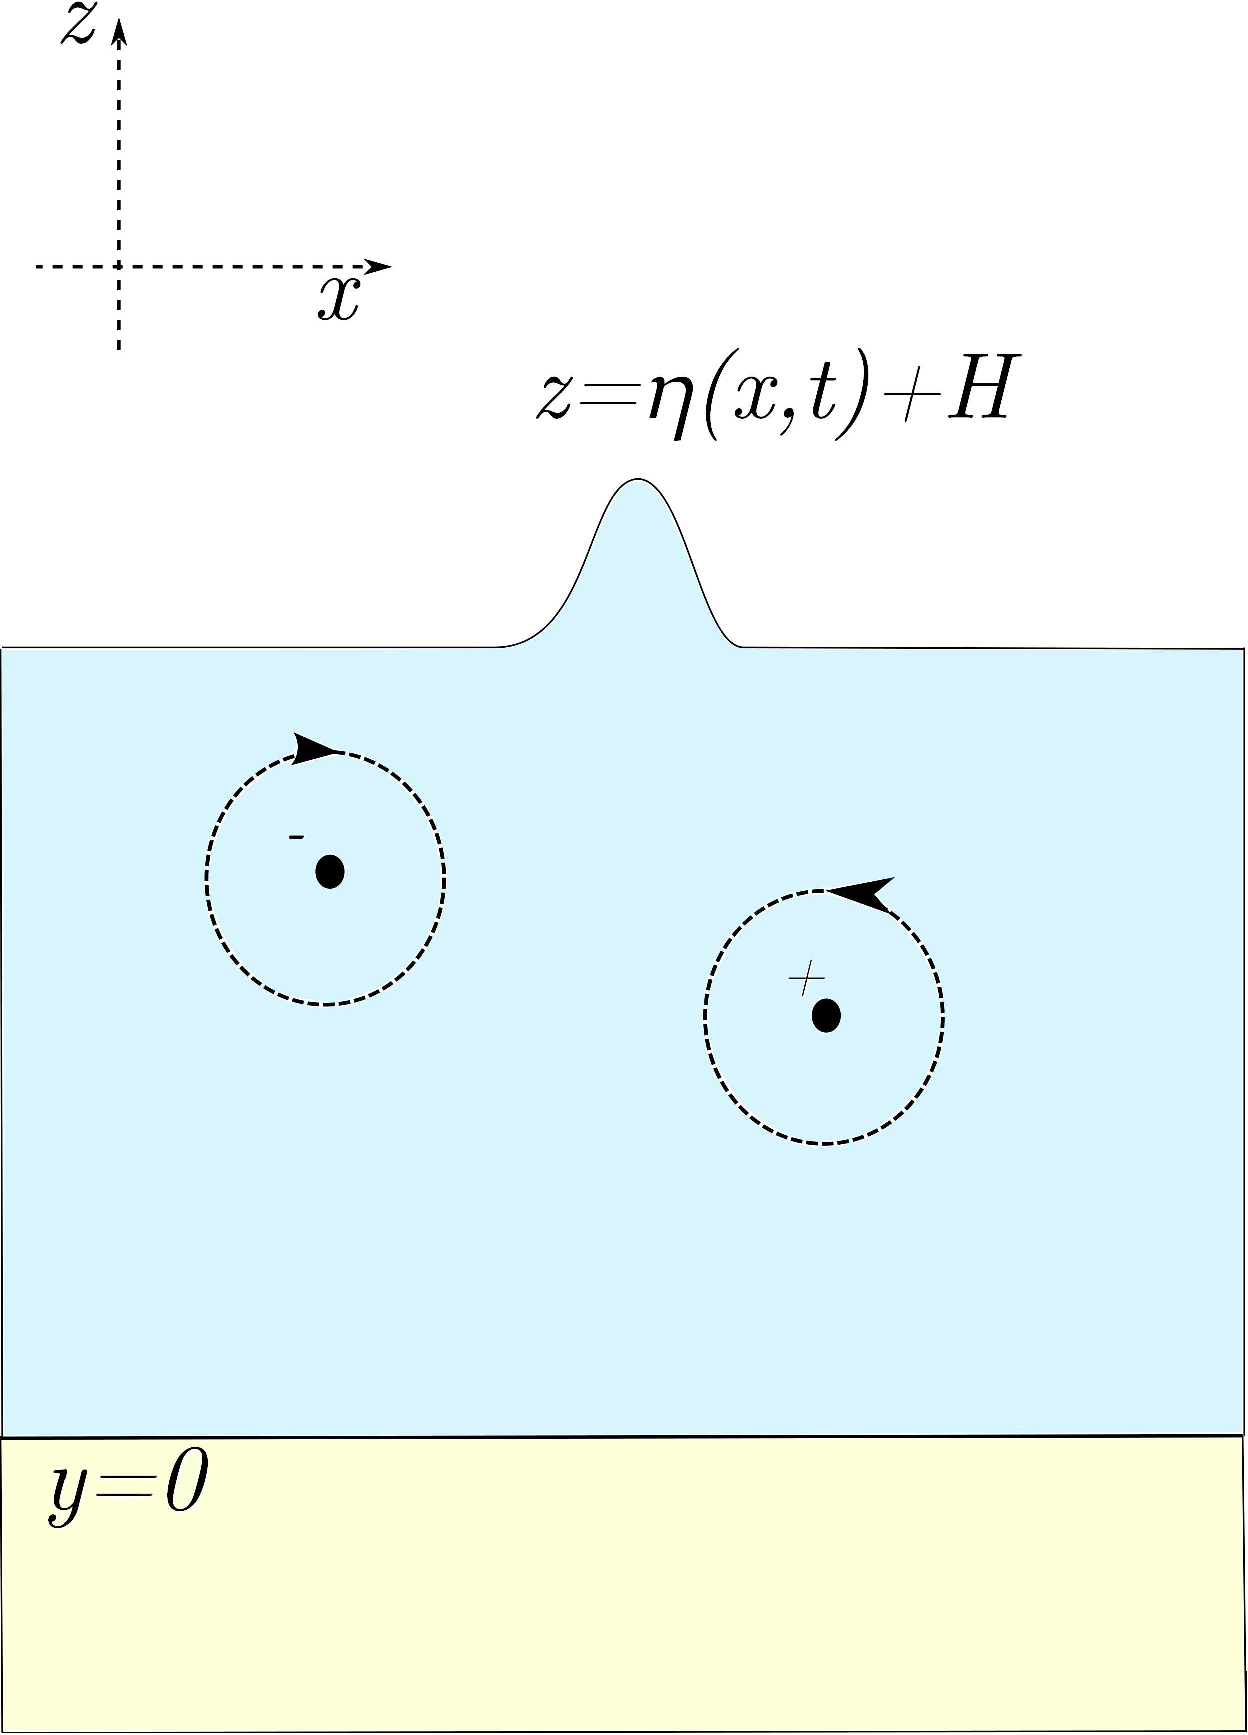
\includegraphics[width=.25\textwidth]{surface_vortex}
\caption{An irrotational point vortex submerged under a free surface gravity wave.}
\label{fig:vortex}
\end{figure}
See Figure \ref{fig:vortex} for reference.  We take the fluid domain to be periodic, with period $2L$, and $-L\leq x \leq L$.  The potential describing the flow is written as 
\[
\phi(x,z,t) = \phi_{v}(x,z,t) + \tilde{\phi}(x,z,t), 
\]
where
\begin{align*}
 \phi_{v}(x,z,t) = & \frac{1}{2\pi}\sum_{j=1}^{N}\Gamma_{j} \phi_{v,j}(x,z,t),\\
=& \frac{1}{2\pi}\left(\phi_{v}^{+}(x,z,t)-\phi_{v}^{-}(x,z,t)\right),
\end{align*}
where $\Gamma_{j}$ denotes the circulation strength of the vortices and
\[
\phi_{v,j}(x,z,t) = \phi_{v,j}^{+}(x,z,t) - \phi_{v,j}^{-}(x,z,t), 
\]
with
\[
\phi_{v,j}^{+}(x,z,t) = \Phi_{p}(x-x_{j}(t),z-z_{j}(t)), ~ \phi_{v,j}^{-}(x,z,t) = \Phi_{p}(x-x_{j}(t),z+z_{j}(t)).
\]
where
\[
\Phi_{p}(x,z) = \sum_{m=-\infty}^{\infty} \tan^{-1}\left(\frac{z}{x-2m L} \right).
\]
We further suppose that 
\[
\p_{z}\tilde{\phi}(x,0,t) = 0, 
\]
so that there is zero flux through the fluid bottom at $z=0$.  Thus, within the domain $0\leq z \leq \eta(x,t)+H$, we are modeling a collection of irrotational vortices underneath a moving surface. 

In order to take into account the periodically repeating images of the vortices, using Fourier transform arguments, we can show that 
\[
\sum_{m=-\infty}^{\infty}\frac{s}{(t-2m\pi)^{2}+s^{2}} = \frac{\sinh(s)}{2(\cosh(s)-\cos(t))}
\]
and
\[
\sum_{m=-\infty}^{\infty}\frac{t-2m\pi}{(t-2m\pi)^{2}+s^{2}} = \frac{\sin(t)}{2(\cosh(s)-\cos(t))}
\]
Standard arguments then give 
\begin{align*}
\dot{x}_{j} = & \frac{1}{4L}\left(  \Gamma_{j}\mbox{cotanh}\left(\frac{\pi z_{j}}{L} \right)+2\sum_{l\neq j}\Gamma_{l}v_{jl}^{(h)} \right)+ \tilde{\phi}_{x}(x_{j},z_{j},t),\\
\dot{z}_{j} = & \frac{1}{2L}\sinh\left(\frac{\pi}{L}z_{j}\right)\sum_{l\neq j} \Gamma_{l} v_{jl}^{(v)} + \tilde{\phi}_{z}(x_{j},z_{j},t),
\end{align*}
where
\begin{align*}
v_{jl}^{(h)} = & \frac{\sinh\left(\frac{\pi}{L}z_{l}\right)\left(\cosh(\frac{\pi}{L}z_{l})-\cosh(\frac{\pi}{L}z_{j})\cos\left(\frac{\pi}{L}(x_{j}-x_{l})\right)\right)}{\left(\cosh\left(\frac{\pi}{L}(z_{j}-z_{l})\right)-\cos\left(\frac{\pi}{L}(x_{j}-x_{l})\right)\right)\left(\cosh\left(\frac{\pi}{L}(z_{j}+z_{l})\right)-\cos\left(\frac{\pi }{L}(x_{j}-x_{l})\right)\right)}, \\
v_{jl}^{(v)} = & \frac{\sin\left(\frac{\pi}{L}(x_{j}-x_{l})\right)\sinh\left(\frac{\pi}{L}z_{l}\right)}{\left(\cosh\left(\frac{\pi}{L}(z_{j}-z_{l})\right)-\cos\left(\frac{\pi}{L}(x_{j}-x_{l})\right)\right)\left(\cosh\left(\frac{\pi}{L}(z_{j}+z_{l})\right)-\cos\left(\frac{\pi }{L}(x_{j}-x_{l})\right)\right)}.
\end{align*}
Likewise, we have the standard surface relations now modified by the presence of the point vortex, i.e. we have the kinematic condition 
\[
\eta_{t} - \tilde{\phi}_{z} + \eta_{x}\tilde{\phi}_{x} =  P_{v}(x,\eta,t), ~ z =  \eta(x,t)+H,  
\]
where
\[
P_{v}(x,\eta,t) =   \p_{z}\phi_{v} -  \eta_{x}\p_{x}\phi_{v} .
\]
and from the Bernoulli equation, we have 
\[
\tilde{\phi}_{t} + \frac{1}{2 }\left| \nabla \tilde{\phi} \right|^{2} +  \nabla\phi_{v}\cdot \nabla\tilde{\phi} + g\eta = E_{v}(x,\eta,t),
\]
where
\[
E_{v}(x,\eta,t) = \frac{1}{2\pi}\sum_{j=1}^{N}\Gamma_{j}\left(\dot{x}_{j}\p_{x}\phi_{v,j} + \dot{z}_{j} \p_{z}\phi_{v,j}  \right) - \frac{1}{2}\left| \nabla \phi_{v} \right|^{2}.
\]
Defining 
\[
\tilde{q}(x,t) = \tilde{\phi}(x,\eta(x,t)+H,t),
\]
we can transform the derivatives of the potential at the surface via the equations
\[
\left.\bp\tilde{\phi}_{x}\\ \tilde{\phi}_{z}\ep\right|_{z=\eta} = \frac{1}{1+\eta_{x}^{2}}\bp 1 & \eta_{x}\\ \eta_{x} & -1\ep\bp\tilde{q}_{x} \\  -\eta_{t} + P_{v}\ep,
\]
and
\[
\tilde{\phi}_{t} = \tilde{q}_{t}-\tilde{\phi}_{z}\eta_{t},
\]
%%%%%%%%%%%%%%%%%%%%%%%%%%%%%%%%%%%%%%%%%%%%%%%%%%%%%%%%%%%%%%%%%%%%%%%%%%%%%%%%%%

%%%%%%%%%%%%%%%%%%%%%%%%%%%%%%%%%%%%%%%%%%%%%%%%%%%%%%%%%%%%%%%%%%%%%%%%%%%%%%%%%%
\section*{Nonlocal Formulation}
A now standard argument from \cite{afm} leads to the AFM equation 
\[
\int_{-L}^{L} e^{-ik x}\left(\cosh( k(  \eta+H))\left(\eta_{t} - P_{v} \right) + i\tilde{q}_{x}\sinh(k( \eta+H))\right) dx = 0, ~ \forall k = \frac{\pi n}{L}.
\]
We are still left with needing to evaluate the background flow potential $\tilde{\phi}$ at the interior points $(x_{j}, z_{j})$.  To deal with this, we introduce the auxillary harmonic function 
\[
\psi_{s,j} = - \frac{1}{4\pi}\sum_{m=-\infty}^{\infty} \left( \mbox{ln}\left( \tilde{x}_{j,m}^{2} + \tilde{z}_{j,-}^{2}  \right) + \mbox{ln}\left( \tilde{x}_{j,m}^{2} + \tilde{z}_{j,+}^{2} \right)\right).
\]
where
\[
\tilde{x}_{j,m} = \frac{(x-x_{j}-2mL)}{L}, ~ \tilde{z}_{j,-} = \frac{\gamma}{H}(z-z_{j}), ~ \tilde{z}_{j,+} = \frac{\gamma}{H}(z+z_{j}),
\]
and
\[
\gamma = \frac{H}{L}.
\]

Our choice of auxillary harmonic function ensures that $\p_{z}\psi_{s,j}(x,0,t)=0$.  Taking $D_{\epsilon}$ to be an open bounded domain that surrounds but does not enclose the point vortices $(x_{j},z_{j})$, using Green's third identity, we have that 
\[
0 =  \int_{D_{\epsilon}}\left(\psi_{s}\Delta \tilde{\phi}_{x} - \tilde{\phi}_{x}\Delta\psi_{s} \right) dA =  \oint_{\p D_{\epsilon}} \left(\psi_{s}\p_{\hat{{\bf n}}}\tilde{\phi}_{x}-\tilde{\phi}_{x}\p_{\hat{{\bf n}}}\psi_{s} \right) ds,
\]
Note, if $\tilde{\phi}$ is harmonic, then so are all of its partial derivatives.  Taking $\epsilon \rightarrow 0^{+}$, we note that for a disc, say $C_{\epsilon}({\bf x}_{j})$  around the point vortex $(x_{j},z_{j})$ that 
\[
 \oint_{C_{\epsilon}({\bf x}_{j})} \left(\psi_{s,j}\p_{\hat{{\bf n}}}\tilde{\phi}_{x}-\tilde{\phi}_{x}\p_{\hat{{\bf n}}}\psi_{s,j} \right) ds =  \epsilon\int_{0}^{2\pi}\left.\left(\psi_{s,j}\p_{r}\tilde{\phi}_{x}- \tilde{\phi}_{x}\p_{r}\psi_{s,j} \right)\right|_{r=\epsilon} d\theta, 
\]
where in the disc we have 
\[
x = x_{j} + L r\cos(\theta), ~ z = z_{j} +  L r\sin(\theta).
\]
Thus, in the limit of $\epsilon\rightarrow 0^{+}$, we get the result 
\[
\oint_{C_{\epsilon}({\bf x}_{j})} \left(\psi_{s,j}\p_{\hat{{\bf n}}}\tilde{\phi}_{x}-\tilde{\phi}_{x}\p_{\hat{{\bf n}}}\psi_{s,j} \right) ds =\tilde{\phi}_{x}(x_{j},z_{j},t).
\]
Likewise, around the discs $C_{\epsilon}({\bf x}_{k})$, $k\neq j$, we have that 
\[
 \oint_{C_{\epsilon}({\bf x}_{k})} \left(\psi_{s,j}\p_{\hat{{\bf n}}}\tilde{\phi}_{x}-\tilde{\phi}_{x}\p_{\hat{{\bf n}}}\psi_{s,j} \right) ds = \epsilon\int_{0}^{2\pi}\left(\psi_{s,j}\p_{r}\tilde{\phi}_{x}- \tilde{\phi}_{x}\p_{r}\psi_{s,j} \right)d\theta, 
\]
where we now take 
\[
x = x_{k} + L r\cos(\theta), ~ z = z_{k} +  L r\sin(\theta).
\]
In this case though, each function in the integrand is continuous over the disc $C_{\epsilon}({\bf x}_{k})$, and thus as $\epsilon \rightarrow 0^{+}$, the contributions from these integrals vanish.  

A standard argument then lets us write 
\[
\int_{-L}^{L}\left.\left(\psi_{s,j}\left(- \eta_{x}\tilde{\phi}_{xx}+\tilde{\phi}_{xz}\right)-\tilde{\phi}_{x}\left(-\eta_{x}\p_{x}\psi_{s,j}+\p_{z}\psi_{s,j}\right) \right)\right|_{z= \eta+H} dx  = \tilde{\phi}_{x}(x_{j},z_{j},t),
\]
since
\[
\p_{z}\psi_{s,j}(x,0,t) = 0, ~ \tilde{\phi}_{xz}(x,0,t) = 0.
\]
Using the identity
\[
\p_{x}\left(\tilde{\phi}_{z}(x, \eta+H,t) \right) = -\eta_{x}\tilde{\phi}_{xx} + \tilde{\phi}_{xz},
\]
we then have 
\[
\tilde{\phi}_{x}(x_{j},z_{j},t) = -\int_{-L}^{L} \left.\left(\tilde{\phi}_{z}\left(\p_{x}\psi_{s,j}+ \eta_{x}\p_{z}\psi_{s,j}\right)+\tilde{\phi}_{x}\left(-\eta_{x}\p_{x}\psi_{s,j} + \p_{z}\psi_{s,j} \right) \right)\right|_{z=\eta+H}dx.
\]
Transforming to surface variables then gives
\[
\tilde{\phi}_{x}(x_{j},z_{j},t) = \int_{-L}^{L}\left.\left(\left(P_{v}-\eta_{t}\right)\p_{x}\psi_{s,j} - \tilde{q}_{x}\p_{z}\psi_{s,j} \right) \right|_{z=\eta+H} dx
\]

Proceeding in the same fashion for $\tilde{\phi}_{z}$, we find
\[
\int_{-L}^{L}\left.\left( \psi_{s,j}\left(-\eta_{x}\tilde{\phi}_{xz}-\tilde{\phi}_{xx}\right)-\tilde{\phi}_{z}\left(-\eta_{x}\p_{x}\psi_{s,j}+\p_{z}\psi_{s,j}\right) \right)\right|_{z=\eta+H} dx  = \tilde{\phi}_{z}(x_{j},z_{j},t),
\]
where we have used the fact that $\tilde{\phi}_{zz} = -\tilde{\phi}_{xx}$.  Integrating by parts then gives 
\[
\tilde{\phi}_{z}(x_{j},z_{j},t) = \int_{-L}^{L}\left.\left(\tilde{\phi}_{x}\left(\p_{x} \psi_{s,j}+ \eta_{x}\p_{z} \psi_{s,j}\right) -\tilde{\phi}_{z}\left(-\eta_{x}\p_{x} \psi_{s,j}+\p_{z}\psi_{s,j}\right)\right)\right|_{z=\eta+H}dx,
\]
which can be shown to yield
\[
\tilde{\phi}_{z}(x_{j},z_{j},t) = \int_{-L}^{L}\left.\left( \left(P_{v}-\eta_{t}\right)\p_{z}\psi_{s,j} + \tilde{q}_{x}\p_{x}\psi_{s,j} \right)\right|_{z=\eta+H} dx.
\]
Thus,we get the following dynamical system for the motion of the vortices:
\begin{align*}
\dot{x}_{j} = & \frac{1}{4L}\left(  \Gamma_{j}\mbox{cotanh}\left(\frac{\pi z_{j}}{L} \right)+2\sum_{l\neq j}\Gamma_{l}v_{jl}^{(h)} \right)\\
&  +\int_{-L}^{L}\left.\left(\left(P_{v} -\eta_{t}\right)\p_{x}\psi_{s,j} - \tilde{q}_{x}\p_{z}\psi_{s,j} \right)\right|_{z=\eta + H} dx\\
\dot{z}_{j} = &  \frac{1}{2L}\sinh\left(\frac{\pi}{L}z_{j}\right)\sum_{l\neq j} \Gamma_{l} v_{jl}^{(v)}\\
&  + \int_{-L}^{L}\left.\left( \left(P_{v} -\eta_{t}\right)\p_{z}\psi_{s,j} + \tilde{q}_{x}\p_{x}\psi_{s,j} \right)\right|_{z=\eta + H} dx.
\end{align*}
%%%%%%%%%%%%%%%%%%%%%%%%%%%%%%%%%%%%%%%%%%%%%%%%%%%%%%%%%%%%%%%%%%%%%%%%%%%%%%%%%%
%%%%%%%%%%%%%%%%%%%%%%%%%%%%%%%%%%%%%%%%%%%%%%%%%%%%%%%%%%%%%%%%%%%%%%%%%%%%%%%%%%
\section*{Scalings and Numerics}
While an expansion approach in terms of the Hamiltonians is desirable, we argue that this process is much more readily done using the nonlocal AFM equations derived above.  We choose the following non-dimesionalizations 
\[
\tilde{x} = \frac{x}{L}, ~\tilde{z} = \frac{z}{H}, ~ \tilde{t} = \frac{H}{d}\frac{\Gamma}{L^{2}} t, ~ \eta = d\tilde{\eta}, ~ \tilde{\phi} = \Gamma \tilde{\tilde{\phi}},
\]
and the non-dimensional parameters
\[
\mu= \frac{d}{H}, ~ \gamma = \frac{H}{L}.
\]
We define the Froude number to be 
\[
F = \frac{\Gamma}{\mu L \sqrt{gH}},
\]
and we define $Q = \tilde{q}_{x}$ so that the Bernoulli equation becomes 
\begin{align*}
Q_{t} + \frac{1}{F^{2}}\eta_{x} + \mu\p_{x}\frac{1}{1+ \mu^{2}\gamma^{2}\eta_{x}^{2}} \left( \frac{1}{2}Q^{2} - \mu \gamma^{2}\eta_{t}\eta_{x}Q  +  \p_{x}\phi_{v} (Q + \mu\gamma\eta_{x}( P_{v}-\gamma\eta_{t}))   \right. \\
\left.\left. + \frac{1}{2}\left(P_{v}^{2}-\gamma^{2}\eta_{t}^{2} \right)+ \p_{z}\phi_{v}\left(\gamma \mu \eta_{x}Q-\left(P_{v}-\gamma \eta_{t}\right) \right) \right)\right|_{z=\mu\eta+1}= \p_{x}E_{v}(x,\mu\eta+1,t),
\end{align*}
where, in the first case,
\[
P_{v}(x,z,t) = \sum_{j=1}^{N} \Gamma_{j} \left(\varphi_{z}(x-x_{j},z;z_{j})-\mu\gamma \eta_{x}\varphi_{x}(x-x_{j},z;z_{j}) \right),
\]
\[
\p_{z}\phi_{v}(x,z,t) =  \sum_{j=1}^{N} \Gamma_{j}\varphi_{z}(x-x_{j},z;z_{j}),
\]
\[
\p_{x}\phi_{v}(x,z,t) = \sum_{j=1}^{N}\Gamma_{j}\varphi_{x}(x-x_{j},z;z_{j}),
\]
where
\[
\varphi_{z}(x,z;z_{j}) = \frac{\sin(\pi x)\sinh(\pi \gamma z)\sinh(\pi \gamma z_{j})}{2\left(\cosh(\pi\gamma(z-z_{j}))-\cos(\pi x)\right) \left(\cosh(\pi\gamma(z+z_{j}))-\cos(\pi x)\right)}
\]
\[
\varphi_{x}(x,z;z_{j}) = \frac{\sinh(\pi \gamma z_{j})\left(\cosh(\pi \gamma z_{j})-\cosh(\pi \gamma z)\cos(\pi x)\right)}{2\left(\cosh(\pi\gamma(z-z_{j}))-\cos(\pi x)\right) \left(\cosh(\pi\gamma(z+z_{j}))-\cos(\pi x)\right)}
\]
and
\[
E_{v}(x,1+\mu\eta,t) = \left.\left(\sum_{j=1}^{N}\Gamma_{j}\left(\dot{x}_{j}\varphi_{x}(x-x_{j},z;z_{j}) + \gamma\dot{z}_{j}\varphi_{z}(x-x_{j},z;z_{j}) \right) -\frac{\mu}{2}\left|\nabla\phi_{v} \right|^{2}\right)\right|_{z=1+\mu \eta}.
\]
The AFM equations become for the surface 
\begin{align*}
\int_{-1}^{1} e^{-i\pi k x}\left(\cosh\left( \pi\gamma k (1 + \mu \eta)\right)\left(\eta_{t} - \frac{1}{\gamma}P_{v}(x,1+\mu\eta,t) \right) \right.\\
\left.+i  \frac{1}{\gamma}Q\sinh\left(\pi \gamma k (1 + \mu \eta)\right)\right) dx = 0,~k\in\mathbb{Z},
\end{align*}
and for the positions of the vortices
\begin{align*}
\dot{x}_{j} = &\frac{\mu }{4}\left(\Gamma_{j}\mbox{cotanh}\left(\pi \gamma z_{j} \right)+2\sum_{l\neq j}\Gamma_{l}v_{jl}^{(h)} \right)\\
&  +\mu\int_{-1}^{1}\left.\left( \left(P_{v} - \gamma \eta_{t}\right)\p_{x}\psi_{s,j} -  Q \p_{z}\psi_{s,j} \right)\right|_{z=\mu\eta + 1} dx\\
\dot{z}_{j} = & \frac{\mu}{2\gamma}\sinh\left( \pi \gamma z_{j}\right)\sum_{l\neq j} \Gamma_{l} v_{jl}^{(v)}\\
&  +  \frac{\mu}{\gamma }\int_{-1}^{1}\left.\left( \left(P_{v} - \gamma \eta_{t}\right)\p_{z}\psi_{s,j} + Q \p_{x}\psi_{s,j} \right)\right|_{z= \mu \eta + 1} dx.
\end{align*}
\subsection*{Dirichlet-to-Neumann Expansions}
Our choice of scaling allows us to readily generate the DNO expansion.  This is done by supposing that 
\[
\eta_{t} - \frac{1}{\gamma}P_{v}(x,1+\mu \eta,t) = \left(G_{0} + \mu G_{1} + \mu^{2}  G_{2} + \cdots \right)Q, 
\]
so that we then get 
\[
\hat{G}_{0}(k) = -\frac{i}{\gamma}\tanh(\pi \gamma k),
\]
\[
G_{1}q = -\gamma^{2}\p_{x}G_{0}(\eta G_{0}Q) - \p_{x}(\eta Q),
\]
and, for $m\geq 1$, 
\begin{align*}
G_{m}q = & -\sum_{j=1}^{\lfloor{m/2}\rfloor}\frac{1}{(2j)!}D^{2j}_{\gamma}\left(\eta^{2j}G_{m-2j}q\right) \\
& - \gamma^{2}\p_{x}G_{0} \sum_{j=0}^{\lfloor{(m-1)/2}\rfloor}\frac{D_{\gamma}^{2j}}{(2j+1)!}\left(\eta^{2j+1}G_{m-2j-1}q\right) - \frac{1}{m!}L_{m} \p_{x}D_{\gamma}^{m-1}\left(\eta^{m}q_{x} \right),
\end{align*}
where
\[
\hat{D}_{\gamma} = \pi \gamma k,
\]
and
\[
\hat{L}_{m} = \left\{
\ba{rl}
1,  & m~\mbox{is odd}, \\
i\gamma \hat{G}_{0}(k),  & m~\mbox{is even}.
\ea
\right.
\]
\subsection*{Linear Dynamics}
In order to get at least some short time intuition about the response of the above system, we suppose that $\mu \ll \gamma$, so that in the linear regime we have $\dot{x}_{j}\sim 0$, $\dot{z}_{j}\sim 0$, and 
\[
Q_{t} + \frac{1}{F^{2}}\eta_{x} = 0,
\]
and
\[
\hat{\eta}_{t} -\hat{G}_{0}(k)\hat{Q} = \int_{\mathbb{R}}e^{-i \pi kx} \tilde{P}_{v}dx,
\]

\[
\tilde{P}_{v} = \frac{\gamma\sqrt{2}}{\pi}\sum_{j=1}^{n}\Gamma_{j}z_{j}e^{-i\pi kx_{j}} \frac{x}{(x^{2}+\gamma^{2}(1-z_{j})^{2})(x^{2}+\gamma^{2}(1+z_{j})^{2})} .
\]
We can readily show using a contour integral argument that 
\[
\int_{\mathbb{R}}e^{-i\pi kx} \tilde{P}_{v}dx = -\frac{i}{\sqrt{2}}\sum_{j=1}^{n}\Gamma_{j} \frac{\sinh(\pi \gamma k z_{j})}{\gamma} e^{-i\pi kx_{j}-\pi \gamma |k|}. 
\]
Note, in order for this result to hold, we need to assume that $0\leq z_{j} <1$.  Thus, in frequency space, we get the leading order behavior
\begin{align*}
\bp \hat{Q}(k,t) \\ \hat{\eta}(k,t) \ep = -\frac{i}{\sqrt{2}}\bp i\pi k(\cos(\omega(k)t)-1)/F^{2}\omega(k) \\   \sin(\omega(k)t) \ep \sum_{j=1}^{n}\Gamma_{j}\frac{\sinh(\pi \gamma k z_{j})}{\gamma \omega(k)}e^{-i\pi kx_{j}-\pi \gamma |k|},
\end{align*}
where 
\[
\omega(k) = \sqrt{\frac{ \pi k \tanh(\pi \gamma k)}{ \gamma F^{2}}}.  
\]
Looking at the response to forcing for the surface displacement $\eta(x,t)$, this response, say $R_{s}(x,t)$, can be found from summing across the separate responses due to each vortex.  These responses, say $R_{s,j}$ are found from the sums
\begin{align*}
R_{s,j}(x,t) = \sum_{k=1}^{\infty} \frac{\sin(\omega(k)t)}{\omega(k)}\frac{\sinh(\pi \gamma k z_{j})}{\gamma}e^{-\pi \gamma k}\sin(\pi k (x-x_{j})),
\end{align*}
so that 
\[
R_{s}(x,t) = \sum_{j=1}^{n}\Gamma_{j}R_{s,j}(x,t).
\]
%%%%%%%%%%%%%%%%%%%%%%%%%%%%%%%%%%%%%%%%%%%%%%%%%%%%%%%%%%%%%%%%%%%%%%%%%%%%%%%%%%
\section*{Numerical Results}
%%%%%%%%%%%%%%%%%%%%%%%%%%%%%%%%%%%%%%%%%%%%%%%%%%%%%%%%%%%%%%%%%%%%%%%%%%%%%%%%%%
For all of the following simulations, we use a pseudo-spectral in space and AM2$^{\ast}$ \cite{fornberg} in time method of lines, and choose $\mu=.2$, $\gamma = \sqrt{\mu}$, and $F=1$.  Note, the choice of Froude number $F=1$ puts us in what is described as the `critical case' by several authors, e.g. see \cite{tryggvason}.  Using the DNO expansions, we include up to the 2nd term, i.e. $G_{2}$, so that we truncate terms at $\mathcal{O}((\mu)^{3})$.  This also limits some of the catastrophic cancellation issues associated with using DNO expansions.  Thus, we capture nonlinear effects at the next order to thse seen in  the KdV equation.  For the time scales of interest then, we should be capturing the relevant physics for shallow water dynamics.  The domain is sampled with $K_{M} = 256$ modes giving a grid spacing of $\delta x = 1/128$, while the time step used is $\delta t = 1\times 10^{-3}$, which introduces error on the order of $10^{-6}$.  The Orszag ``2/3-rule'' is used to control aliasing error throughout the simulation.     

%%%%%%%%%%%%%%%%%%%%%%%%%%%%%%%%%%%%%%%%%%%%%%%%%%%%%%%%%%%%%%%%%%%%%%%%%%%%%%%%%%
\subsection*{Interactions with Shallow-Water-Traveling Waves}
By settinig the vortex strengths, $\Gamma_{j}$, to zero, we would expect to limit onto the classical case of shallow water flow in which the KdV equation becomes a valid asymptotic approximation.  Expanding up to $\mathcal{O}(\mu,\gamma^{2})$ we get the system of equations 
\[
\tilde{Q}_{t} + \frac{1}{F^{2}}\eta_{x} + \frac{\mu}{2}\p_{x}Q^{2} \sim 0, 
\]
and
\[
\left(1 - \frac{\gamma^{2}}{2}\p_{x}^{2}\right)\eta_{t} + \p_{x}\left(1-\frac{\gamma^{2}}{6}\p_{x}^{2} \right)Q + \mu \p_{x}(\eta Q) \sim 0.
\]
By rescaling time so that 
\[
\tilde{t} = \frac{1}{F} t,
\]
and introducing the coordinates
\[
\xi = x - \tilde{t}, ~ \tau = \mu \tilde{t}, 
\]
and taking the balance 
\[
\mu = \gamma^{2}, 
\]
allows us to derive the KdV equation
\[
2Q_{\tau} + 3F QQ_{\xi} + \frac{1}{3} Q_{\xi\xi\xi} = 0.
\]
Note, we see by deriving this equation that we are in fact, in the abscence of vortices, in a classicaly defined shallow water regime, thus justifying our choice of scalings {\it a posteori}.  

As is known, the KdV equation has an infinite number of periodic traveling wave solutions of the form 
\[
Q(x,t) \sim \frac{4}{3F} \tilde{m}^{2}\mathcal{K}^2(\tilde{m})\mbox{cn}^{2}\left(\mathcal{K}(\tilde{m}) \left( x- \frac{t}{F} - \frac{2}{3}\mu\mathcal{K}^{2}(\tilde{m}) (2\tilde{m}^{2}-1)t\right);\tilde{m}\right),
\]
where $0\leq \tilde{m}<1$ is the elliptic modulus of the cnoidal function $\mbox{cn}(\cdot;\tilde{m})$ and where $\mathcal{K}(\tilde{m})$ represents the complete elliptic integral of the first kind.  This then implies that the surface profile is to leading order given by 
\[
\eta(x,t) \sim \left(F+\frac{2}{3}\mu F^{2}\mathcal{K}^{2}(\tilde{m})(2\tilde{m}^{2}-1)\right)Q(x,t).
\]
Taking then the elliptic modulus $\tilde{m=.2}$, we look at the case of two counter-propagating vortices under the traveling wave.  We introduce two counter-rotating vortices of strengths $\Gamma_{1}=1$ and $\Gamma_{2}=-1$ starting at positions $x_{1}(0)=-\mu\gamma$ and $x_{2}(0)=\mu\gamma$, and $z_{1}(0)=z_{2}(0)=.25$.  We first set $\Gamma_{1}=.1$ and $\Gamma_{2}=-.1$ while keeping the Froude number $F=1$.  We point out though that given the relatively small choices of the non-dimensionalized circulation strengths, this effectively lowers the Froude number.   

As can be seen from the motion of the vortices in Figures \ref{fig:cnxtrackpt1} and \ref{fig:cnztrackpt1}, for short times, the relatively weak circulations cause the vortices to oscillate.  However, on a longer time scale, the vortices in effect escape and begin to rise, though the oscillatory motion induced in the fluid column by the passing wave causes the vortices to continue to have an oscillatory component to their motion.  We likewise see that the rightward propagation of the wave pushes the right-most vortex in a retrograde fashion towards the left most.  This type of behavior is characteristic of weak vortices, and is similar to the sub-critical phenomena seen in \cite{tyvand2}.
\begin{figure}[!h]
\centering
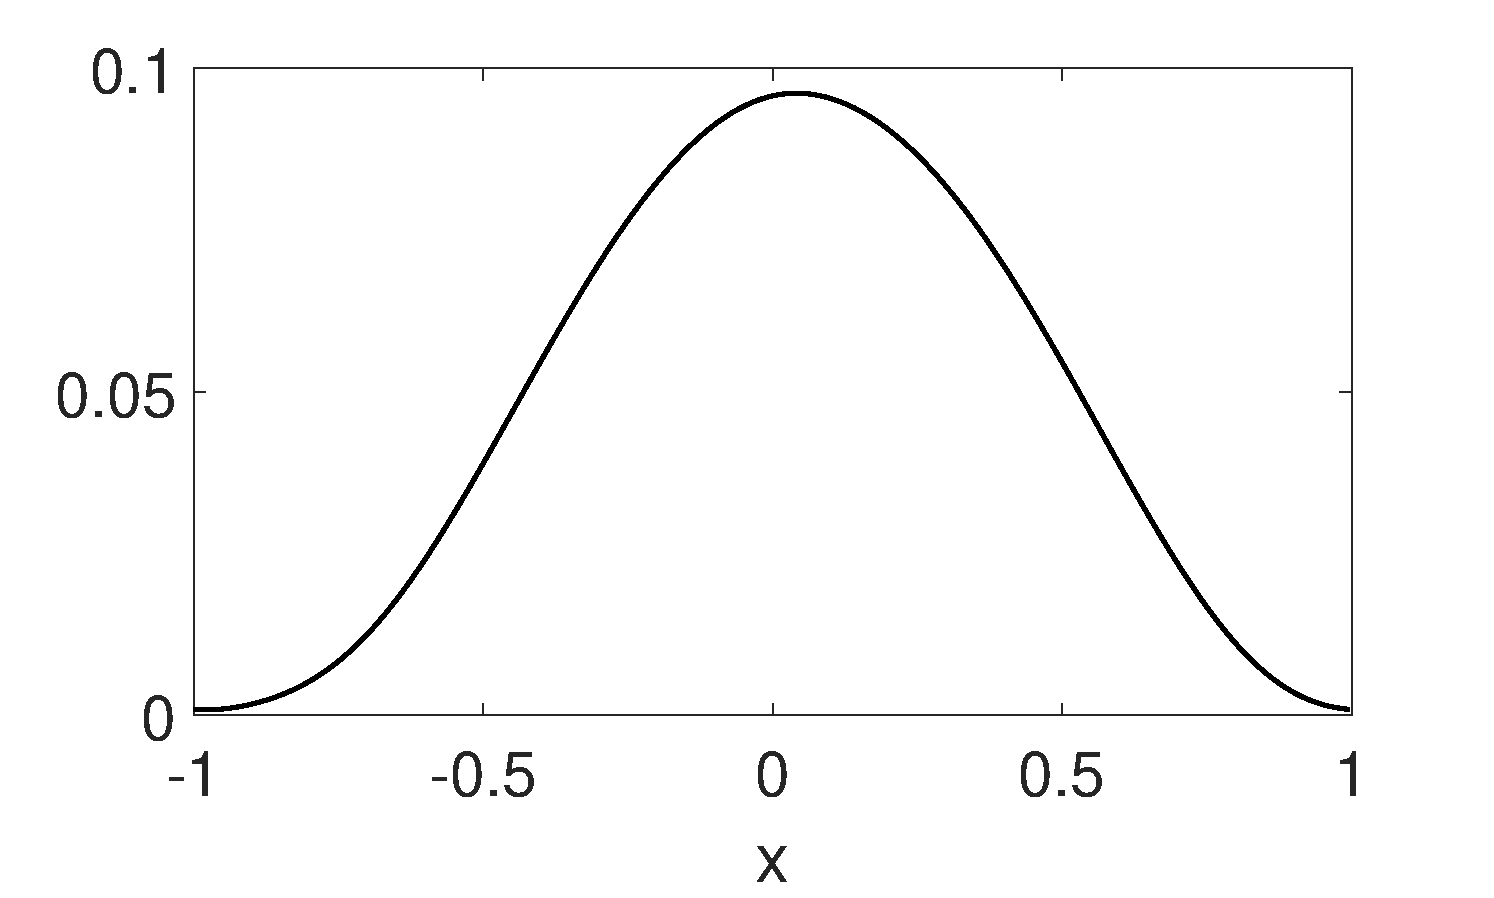
\includegraphics[width=.75\textwidth]{surf_resp_cnoid_mu_pt2_F_1_tf_5_gam_pt1}
\caption{Surface response $\eta(x,5)$ for elliptic modulus $\tilde{m}=.2$.}
\label{fig:surfrepcn}
\end{figure}
\begin{figure}[!h]
\centering
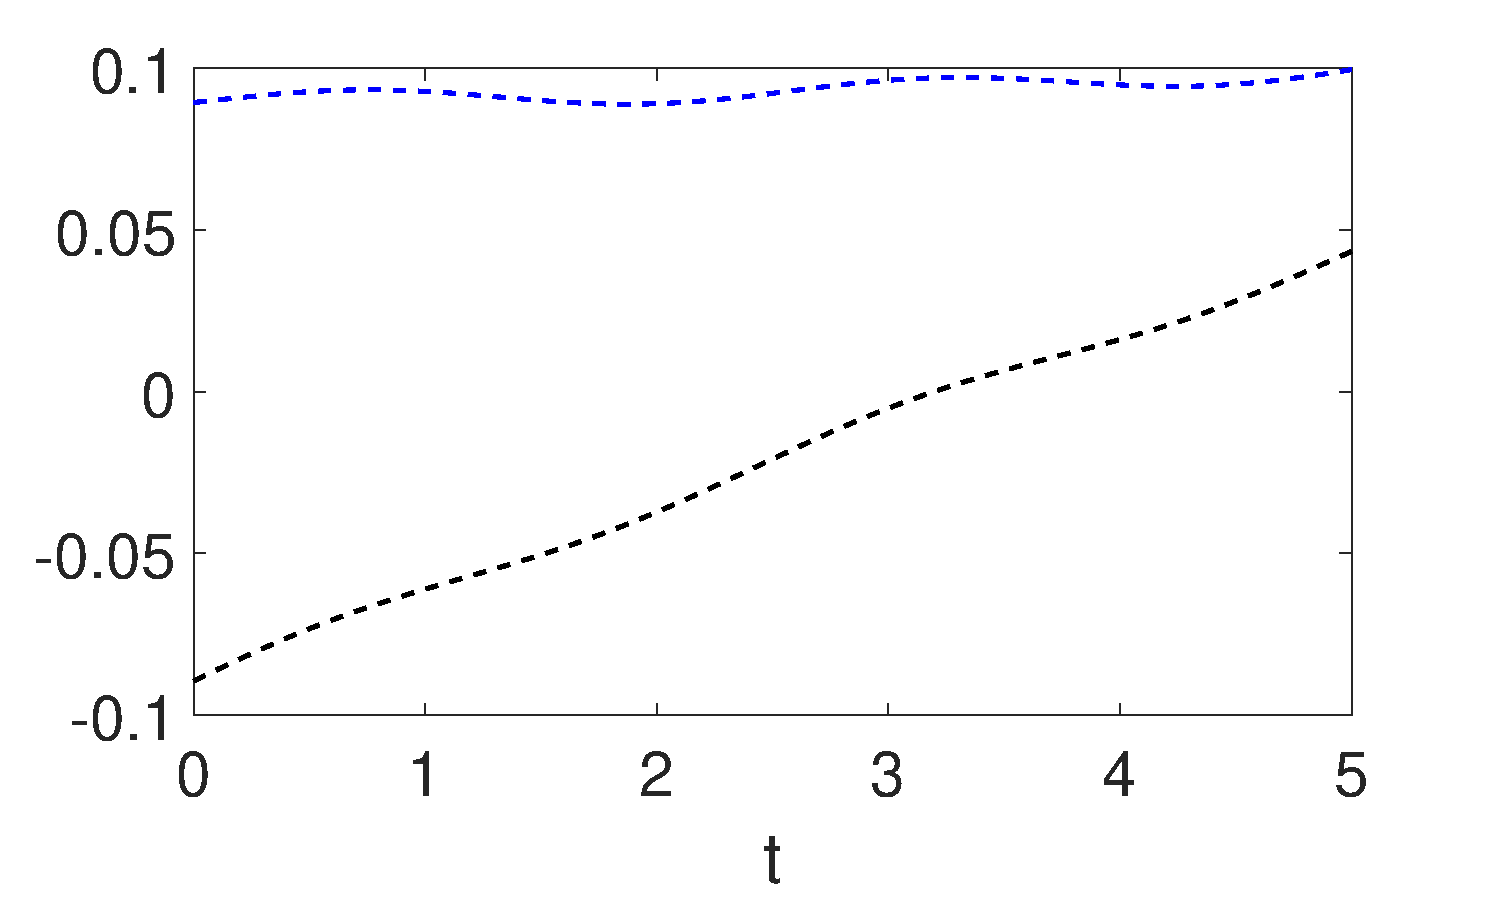
\includegraphics[width=.75\textwidth]{xtrack_cnoid_mu_pt2_F_1_tf_5_gam_pt1}
\caption{Horizontal positions of vortices for $0\leq t \leq 5$.}
\label{fig:cnxtrackpt1}
\end{figure}
\begin{figure}[!h]
\centering
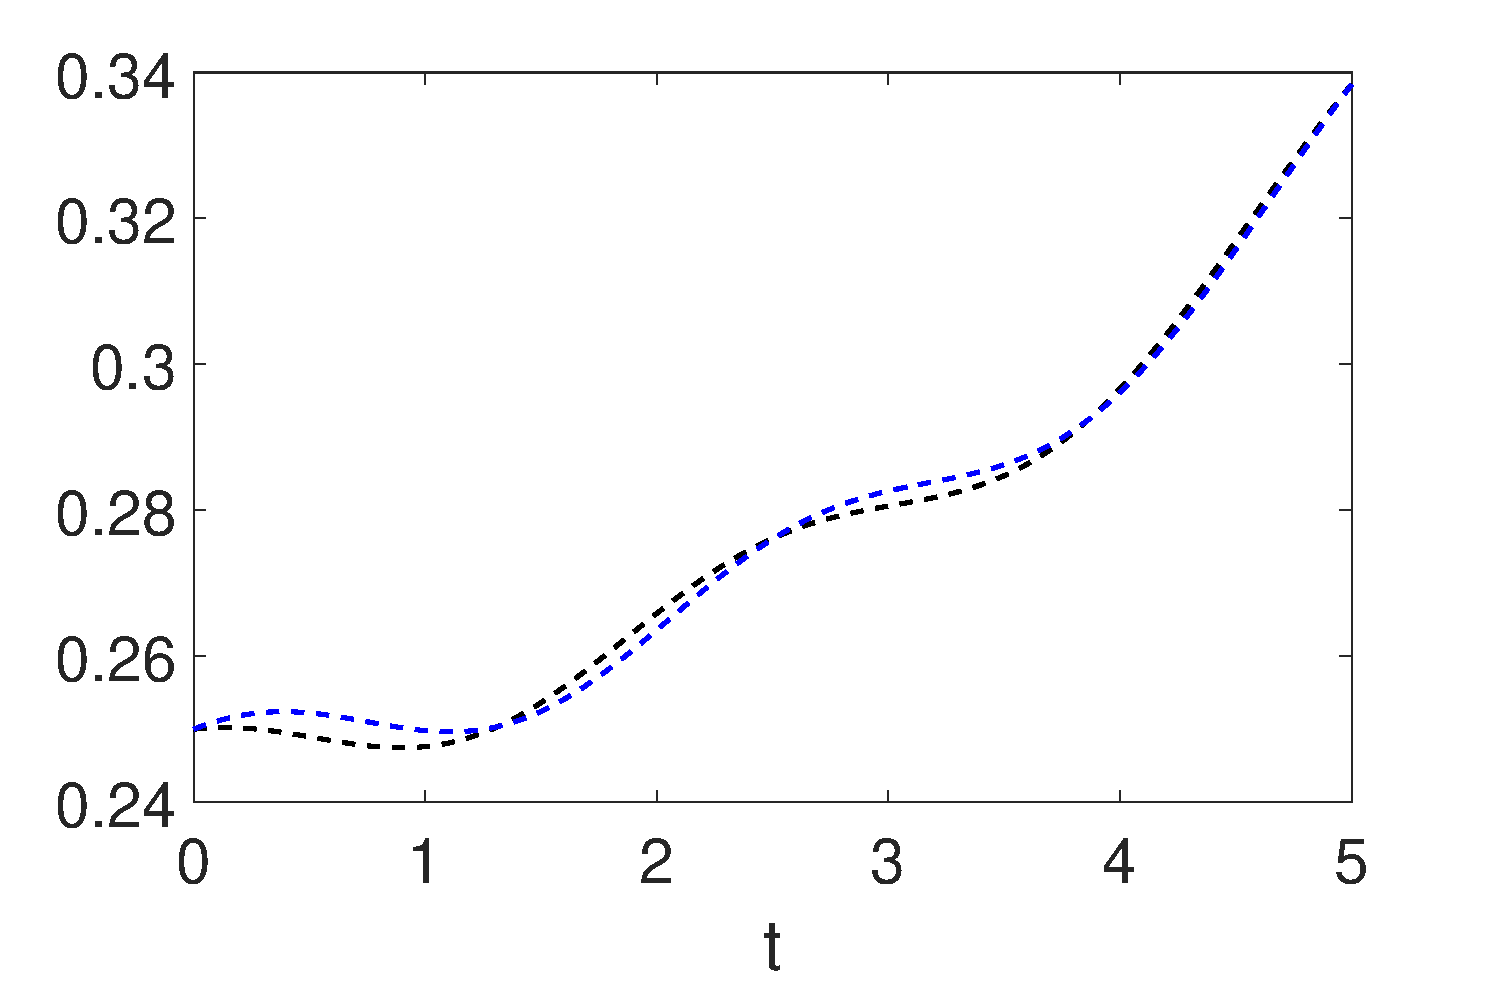
\includegraphics[width=.75\textwidth]{ztrack_cnoid_mu_pt2_F_1_tf_5_gam_pt1}
\caption{Vertical position of vortices for $0\leq t \leq 5$.}
\label{fig:cnztrackpt1}
\end{figure}

%%%%%%%%%%%%%%%%%%%%%%%%%%%%%%%%%%%%%%%%%%%%%%%%%%%%%%%%%%%%%%%%%%%%%%%%%%%%%%%%%%
\subsection*{Two Counter-Propagating Vortices in Shallow Water}

We introduce two counter-rotating vortices of strengths $\Gamma_{1}=1$ and $\Gamma_{2}=-1$ starting at positions $x_{1}(0)=-\mu\gamma$ and $x_{2}(0)=\mu\gamma$, and $z_{1}(0)=z_{2}(0)=.25$.  The surface and velocity potential are both taken to be zero at $t=0$.  The vortex positions are found using a fourth-order Runge-Kutta scheme.  We first look at the surface response up to $t=.1=F$.  Given the relatively short time scale, we compare our numerics to the linear theory derived in the previous section.  For a pair of counter-rotating vortices, we have that the forcing response for the free surface is given by the function
\[
R_{s}(x,t) = 2\sum_{k=1}^{\infty} \frac{\sin(\omega(k)t)}{\omega(k)}\frac{\sinh(\pi \gamma k z_{1})}{\gamma}e^{-\pi \gamma k}\sin(\pi k x_{1})\cos(\pi k x).
\]
We compare this response function to the numerical results in Figure \ref{fig:linrep}.  As can be seen, even up to $t=1$, the linear response is quite accurate.  Further, the falling troughs, or scars, seen in much of the existing literature \cite{marcus,tryggvason} are present.  However, one can also see the beginnings of the break down of the symmetry around the $x=0$ axis. Thus nonlinear effects are becoming apparent for $t = \mathcal{O}(1)$.   We describe this process as `toppling'.  We again point out that in much of the prior literature, symmetry of the flow around the x-axis was enforced in numerical schemes.  This is not the case in our work, and thus we are the first to report this toppling effect.  We do note however that the key features reported in previous literature, such as the surface mound, and the presence of scars are still clearly visible in Figure \ref{fig:linrep}.
\begin{figure}[!h]
\centering
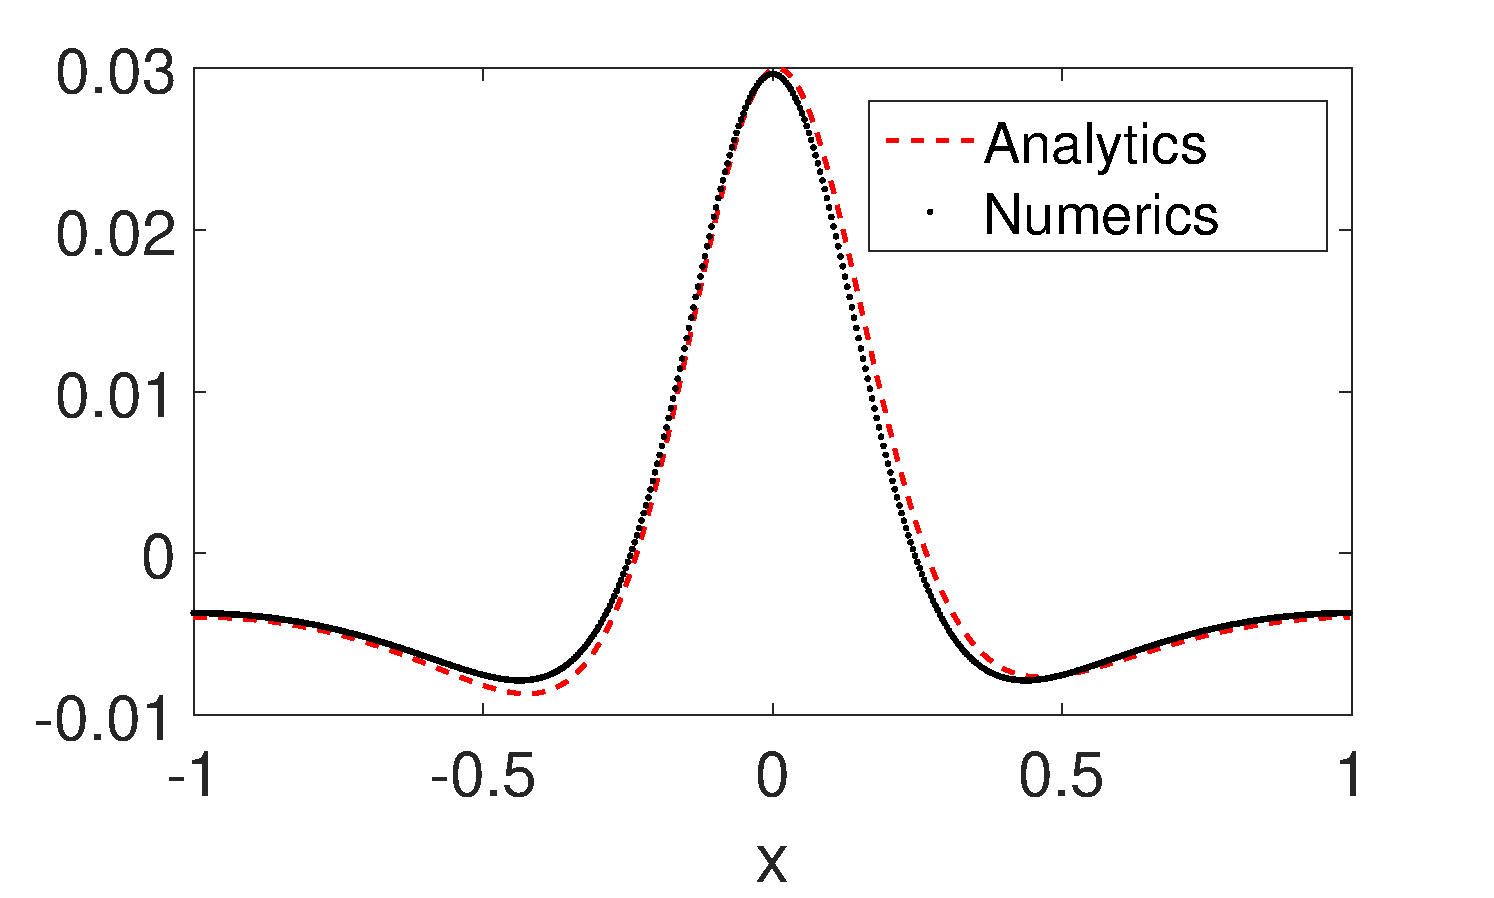
\includegraphics[width=.75\textwidth]{lin_response_tf_pt1}
\caption{Comparison between linear theory and numerics at $t=.1$.}
\label{fig:linrep}
\end{figure}

To further explore the role of nonlinearity, we now look at longer timescales where we let time $t = .7 \sim F$.  As can be seen in Figure \ref{fig:surfrep}, the $x=0$ symmetry has now completely disappeared.  Further, looking at the power spectra at $t=.7$, see Figure \ref{fig:pspec3}, we see that a significant amount of energy has been transported into higher wave numbers as the vortices rise.  This explains then the formation of the step seen in Figure \ref{fig:surfrep}, which represents the onset of wave-breaking.  Longer time simulations show that after $t=.7$, the numerical method breaks down with the appearance of ever higher frequency oscillations, which confirms that the wave would break in physical settings.  
\begin{figure}[!h]
\centering
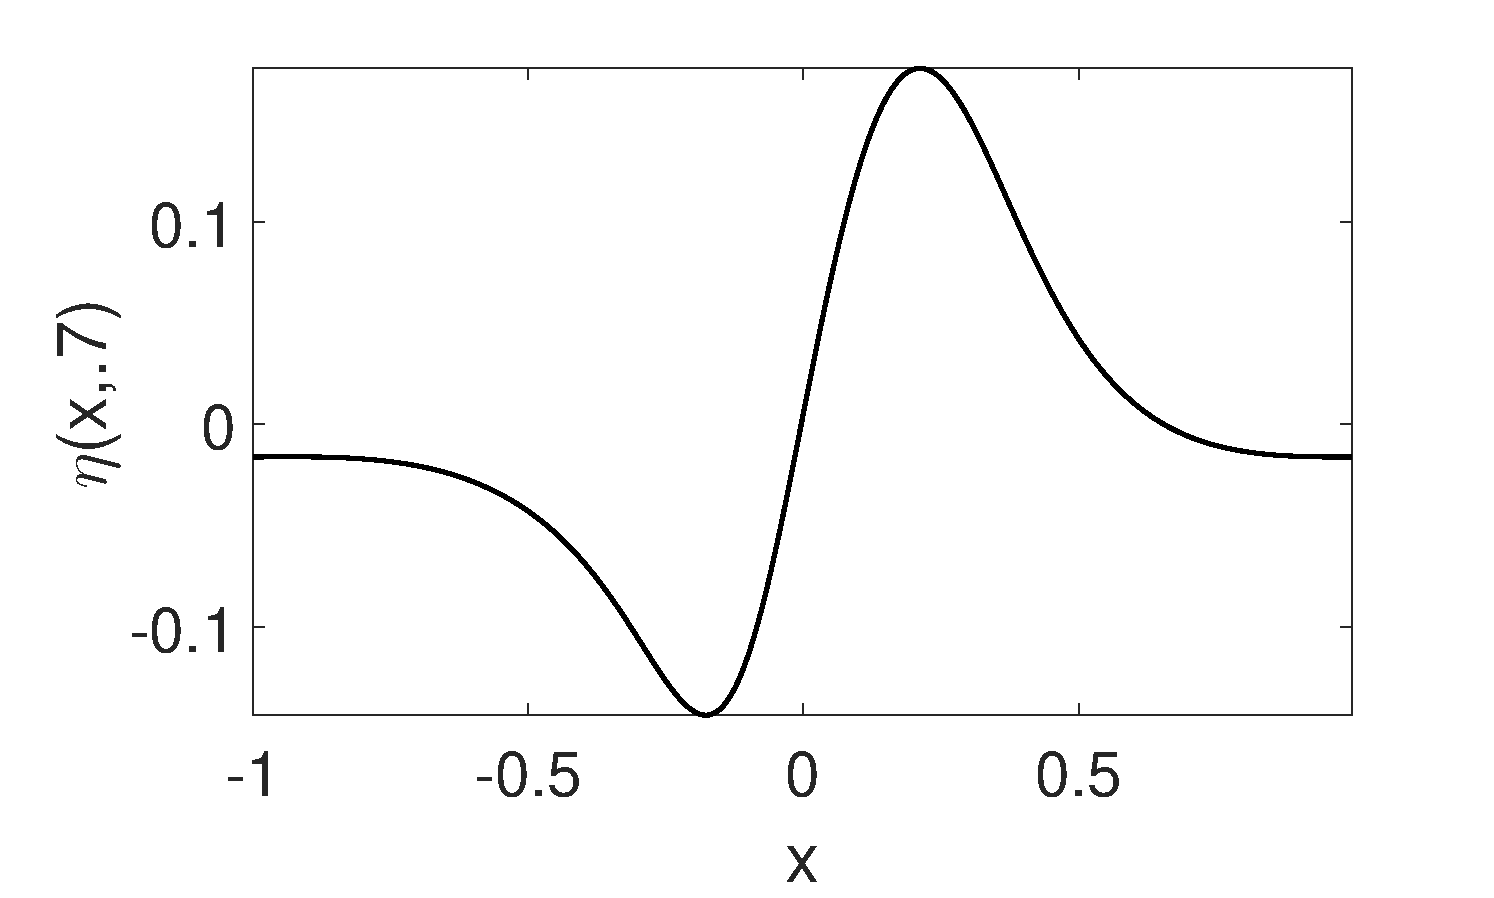
\includegraphics[width=.75\textwidth]{surf_resp_mu_pt2_F_1_tf_pt7}
\caption{Surface response $\eta(x,.7)$ over two counter-propagating vortices.}
\label{fig:surfrep}
\end{figure}
\begin{figure}[!h]
\centering
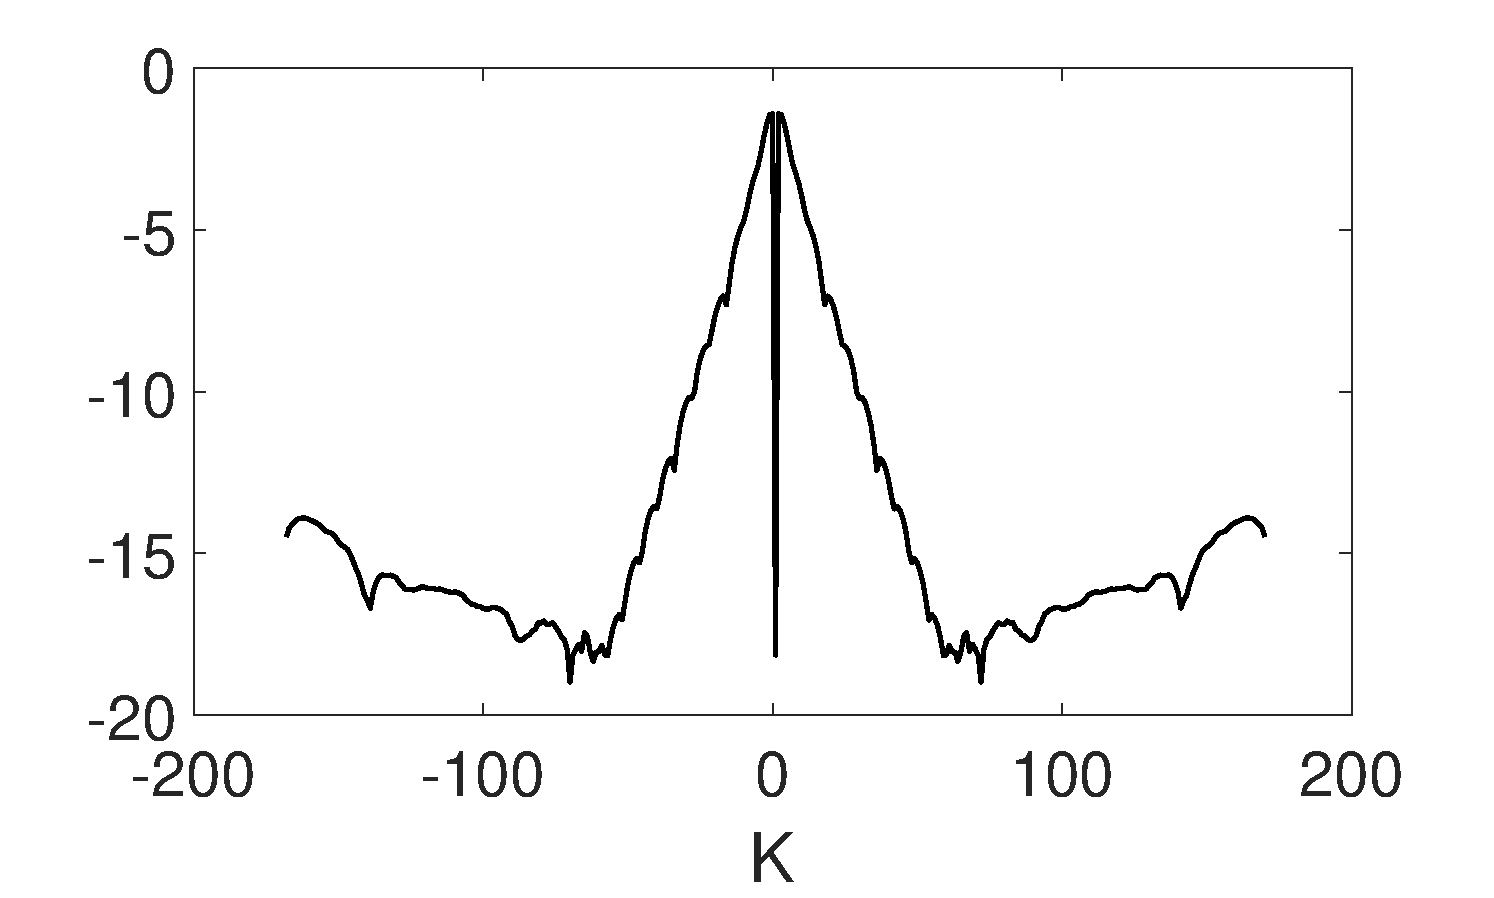
\includegraphics[width=.75\textwidth]{pspec_mu_pt2_F_1_tf_pt7}
\caption{Log plot of the power spectrum at $t = .7$ over wave numbers $-128\leq k \leq 128$.  As can be seen, the rising vortices pump more energy into higher wavenumbers in the surface profile.}
\label{fig:pspec3}
\end{figure}
\begin{figure}[!h]
\centering
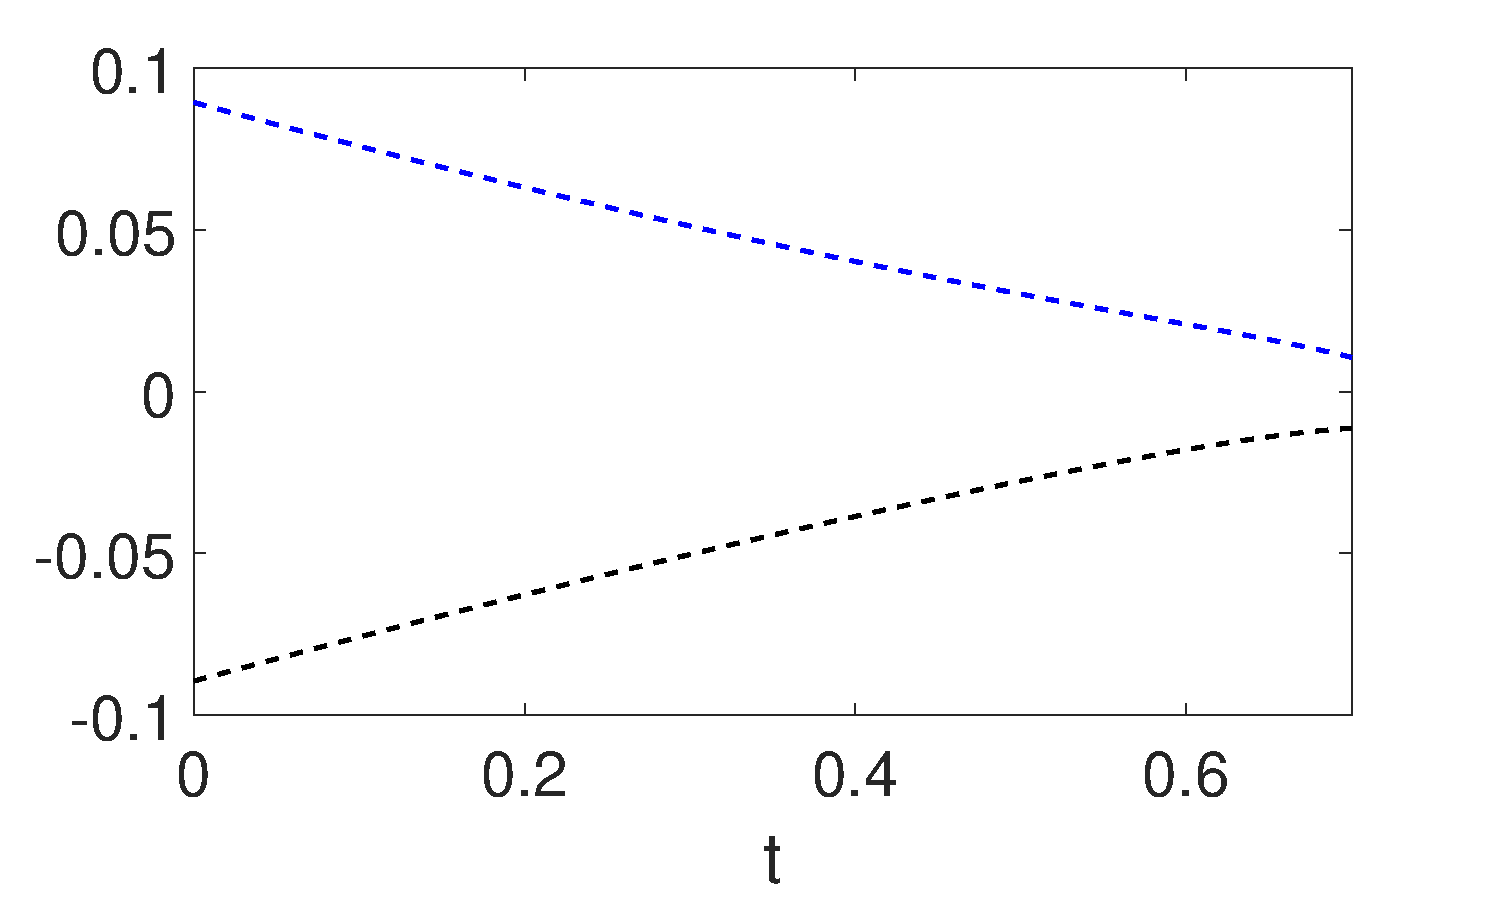
\includegraphics[width=.75\textwidth]{xtrack_mu_pt2_F_1_tf_pt7}
\caption{Horizontal positions of the two vortices for $0\leq t \leq .7$.}
\end{figure}
\begin{figure}[!h]
\centering
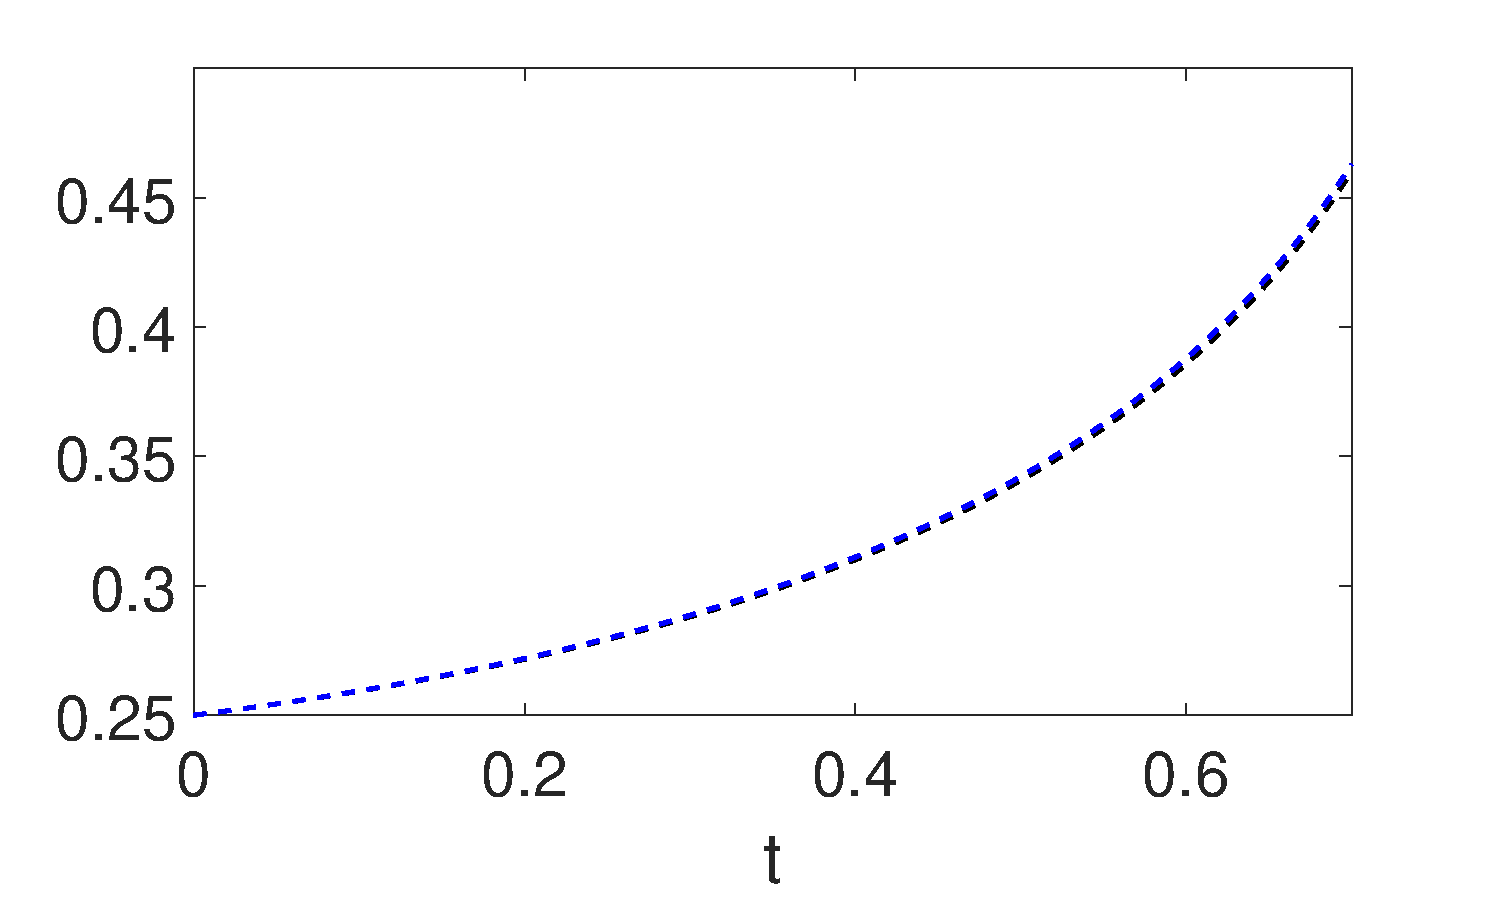
\includegraphics[width=.75\textwidth]{ztrack_mu_pt2_F_1_tf_pt7}
\caption{Vertical position of the two vortices for $0\leq t \leq .7$.}
\end{figure}


\subsection*{A Four Vortex Case}
Using the same numerical scheme and parameters as from above, we now look at the case of four vortices, chosen so that
\[
\Gamma_{1}=\Gamma_{2}=1, ~ \Gamma_{3}=\Gamma_{4}=-1,
\]
\begin{align*}
x_{1}(0)=-2\mu\gamma-\mu\gamma/2, ~ x_{2}(0)=-2\mu\gamma+\mu\gamma/2,\\ x_{3}(0)=2\mu\gamma-\mu\gamma/2, ~ x_{4}(0)=2\mu\gamma+\mu\gamma/2,
\end{align*}
and $z_{j}(0)=.25$.  Looking at the longer time scale where $t=.8$ generates the following figures
\begin{figure}[!h]
\centering
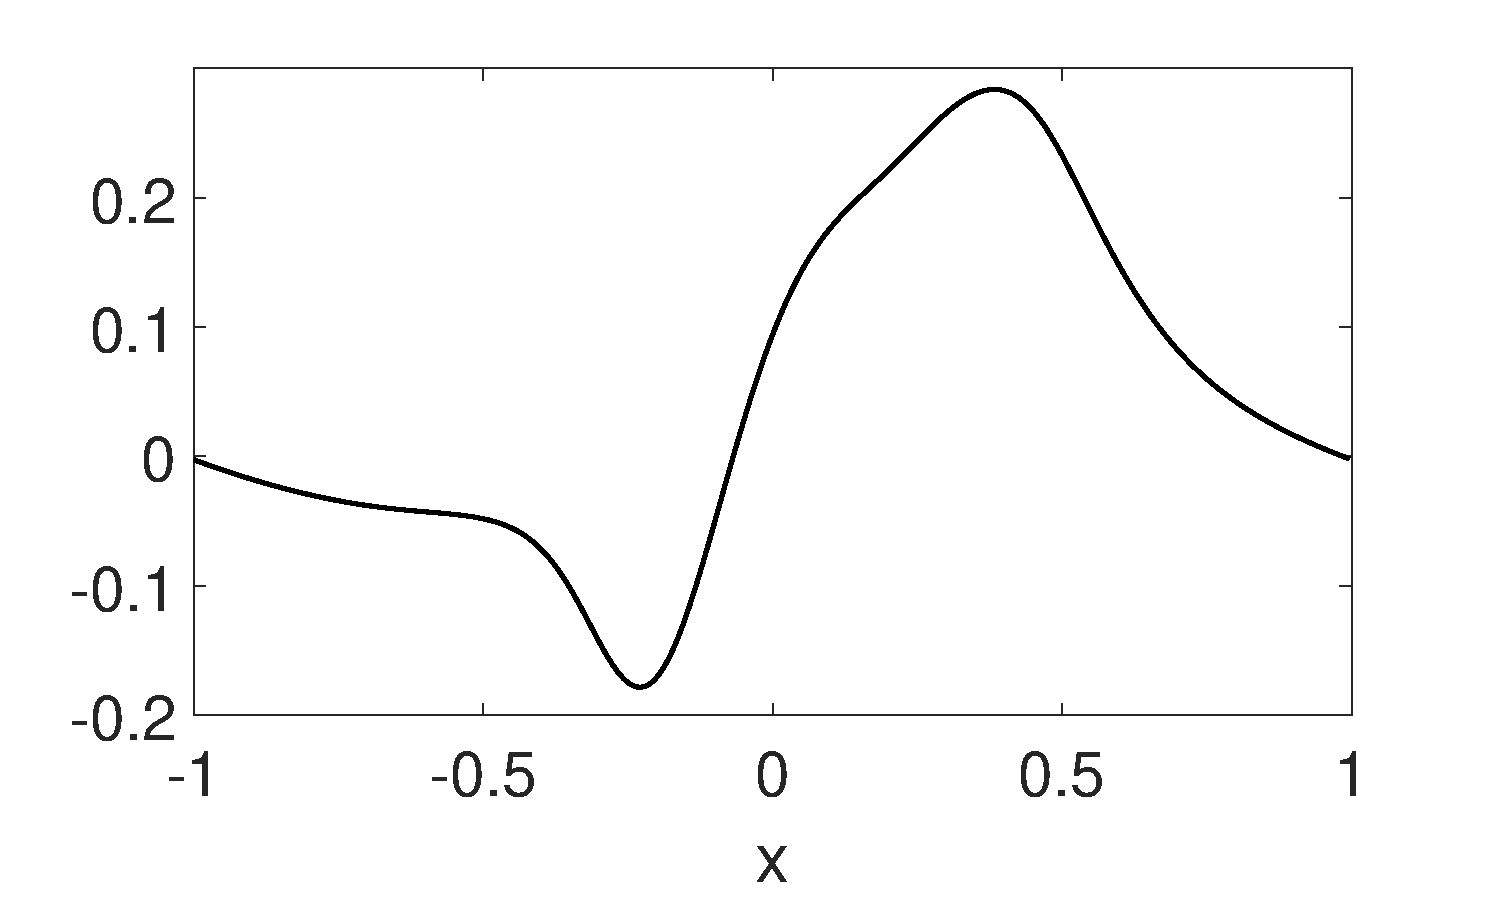
\includegraphics[width=.75\textwidth]{surf_resp_mu_pt2_F_1_tf_pt8_4vort}
\caption{Surface response $\eta(x,.8)$ over four co-rotating and counter-propagating vortices.}
\label{fig:surfrep4}
\end{figure}
\begin{figure}[!h]
\centering
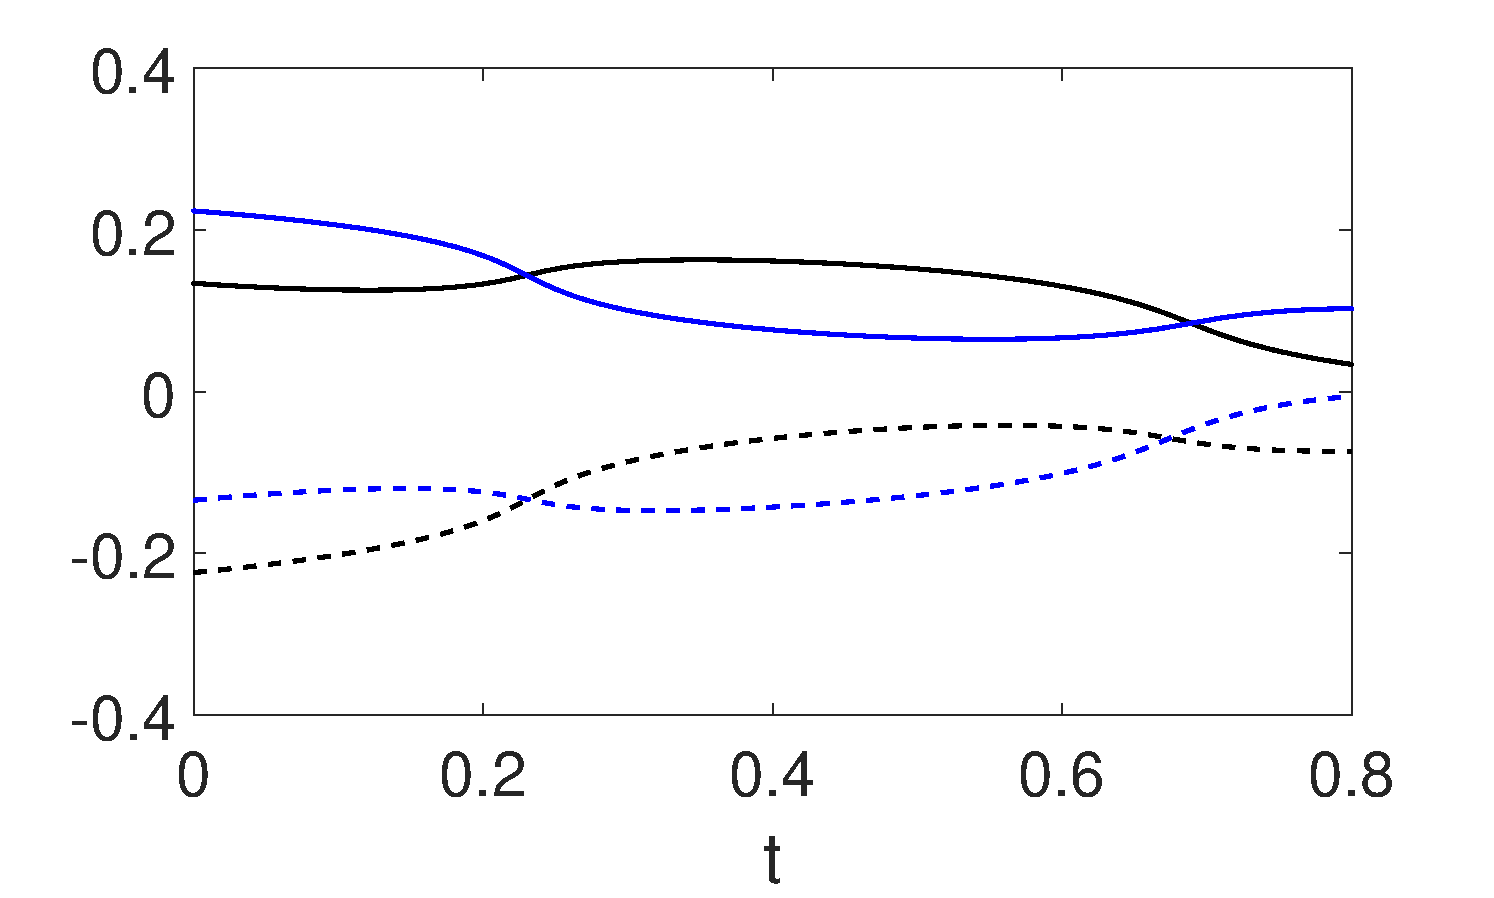
\includegraphics[width=.75\textwidth]{xtrack_mu_pt2_F_1_tf_pt8_4vort}
\caption{Horizontal positions of the four vortices for $0\leq t \leq .8$.}
\end{figure}
\begin{figure}[!h]
\centering
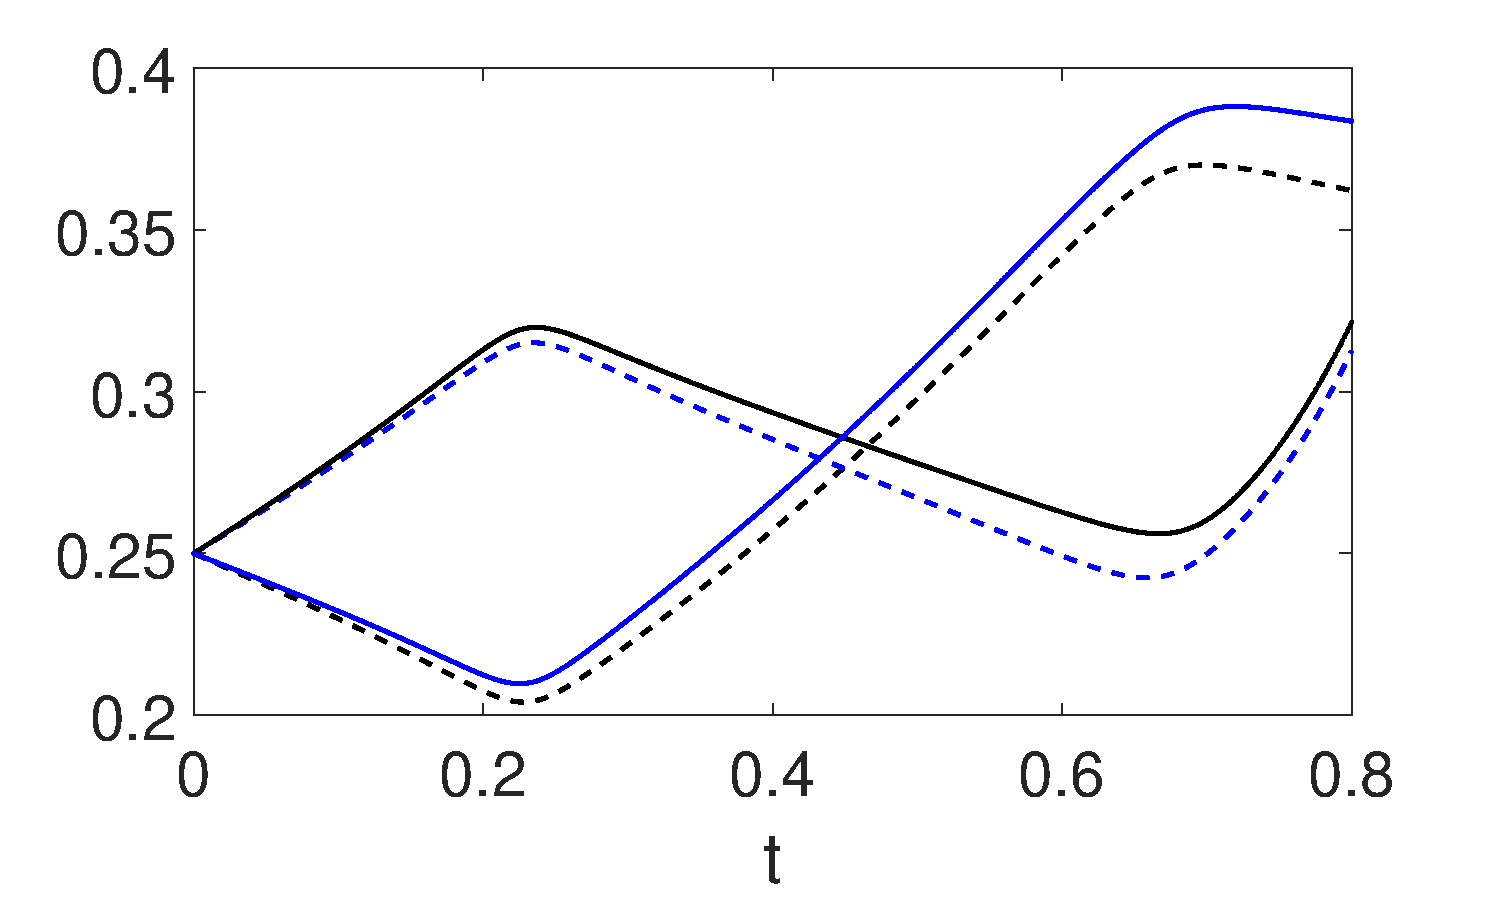
\includegraphics[width=.75\textwidth]{ztrack_mu_pt2_F_1_tf_pt8_4vort}
\caption{Vertical position of vortices for $0\leq t \leq .8$.  This figure shows that the left-most, negatively oriented vortex moves in the vertical with the right-most, positively oriented vortex and vice versa.}
\end{figure}
While still exhibiting the general super-critical behavior one would expect, the dynamics are not far richer, and this is manifested in the surface profile seen in Figure \ref{fig:surfrep4}.
%%%%%%%%%%%%%%%%%%%%%%%%%%%%%%%%%%%%%%%%%%%%%%%%%%%%%%%%%%%%%%%%%%%%%%%%%%%%%%%%%%

%%%%%%%%%%%%%%%%%%%%%%%%%%%%%%%%%%%%%%%%%%%%%%%%%%%%%%%%%%%%%%%%%%%%%%%%%%%%%%%%%%
\bibliography{waves_over_vortices}
\bibliographystyle{unsrt}
\end{document}